\documentclass[12pt]{article}
\usepackage[spanish]{babel}
\usepackage{makeidx}
\usepackage[margin=1in]{geometry}  % set the margins to 1in on all sides
\usepackage{graphicx}              % to include figures
\usepackage{amsmath}               % great math stuff
\usepackage{amsfonts}              % for blackboard bold, etc
\usepackage{amsthm}                % better theorem environments
\usepackage{makeidx}               % index
\usepackage[utf8]{inputenc}        % now we have tildes!
\usepackage{wrapfig}               % images
\usepackage{listings}              % Unordered lists
\usepackage{hyperref}              % hyperlinks
\usepackage{xcolor}                % to colorize font
\usepackage{blindtext}             % to colorize font
\usepackage{caption}
\usepackage{subcaption}

\makeindex

\begin{document}

\begin{titlepage}

\newcommand{\HRule}{\rule{\linewidth}{0.5mm}} % Defines a new command for the horizontal lines, change thickness here

\center % Center everything on the page

%----------------------------------------------------------------------------------------
%	LOGO SECTION
%----------------------------------------------------------------------------------------

\textsc{\LARGE Universidad Carlos III de Madrid}\\[1.2cm] % Name of your university/college

%----------------------------------------------------------------------------------------
%	HEADING SECTIONS
%----------------------------------------------------------------------------------------


\includegraphics[width=9cm]{Logo}\\[1.2cm] % Include a department/university logo - this will require the graphicx package

\textsc{\Large Aprendizaje Automático}\\[0.5cm] % Major heading such as course name
\textsc{\large Grado en Ingeniería Informática}\\[0.6cm] % Minor heading such as course title
\textsc{\large Grupo 83}\\[0.5cm]

%----------------------------------------------------------------------------------------
%	TITLE SECTION
%----------------------------------------------------------------------------------------

\HRule \\[0.7cm]
{ \huge \bfseries Tutorial 4: Introduccíon al aprendizaje por refuerzo}\\[0.4cm] % Title of your document
\HRule \\[0.7cm]

%----------------------------------------------------------------------------------------
%	AUTHOR SECTION
%----------------------------------------------------------------------------------------

\textit{Autores:}\\
Daniel \textsc{Medina García}\\ % Your name
Alejandro \textsc{Rodríguez Salamanca}\\[1.1cm] % Your name

%----------------------------------------------------------------------------------------
%	DATE SECTION
%----------------------------------------------------------------------------------------

{\large \today}\\ % Date, change the \today to a set date if you want to be precise

%----------------------------------------------------------------------------------------

\vfill % Fill the rest of the page with whitespace

\end{titlepage}

\tableofcontents

\newpage
\thispagestyle{empty}
\clearpage
\vspace*{\fill}
\begin{center}
    \begin{minipage}{\textwidth}
        \begin{center}
            \section*{Introducción}
            % TODO: Needed?
        \end{center}
    \end{minipage}
\end{center}
\vfill

\newpage
\section{Ejercicio 1}

En este primer ejercicio tomamos contacto con el programa ejecutando tanto el agente manual como el estándar.
Por cada movimiento ejecutado, en la salida por consola aparecen el estado inicial, la acción tomada, el estado al que se llega y la recompensa obtenida. El agente por defecto es \textit{random}, que toma acciones aleatorias entre las permitidas. La Figura 1 muestra los MDP deterministas requeridos en el enunciado del tutorial:

\begin{figure}[h]
    \centering
    \begin{subfigure}{.5\textwidth}
        \centering
        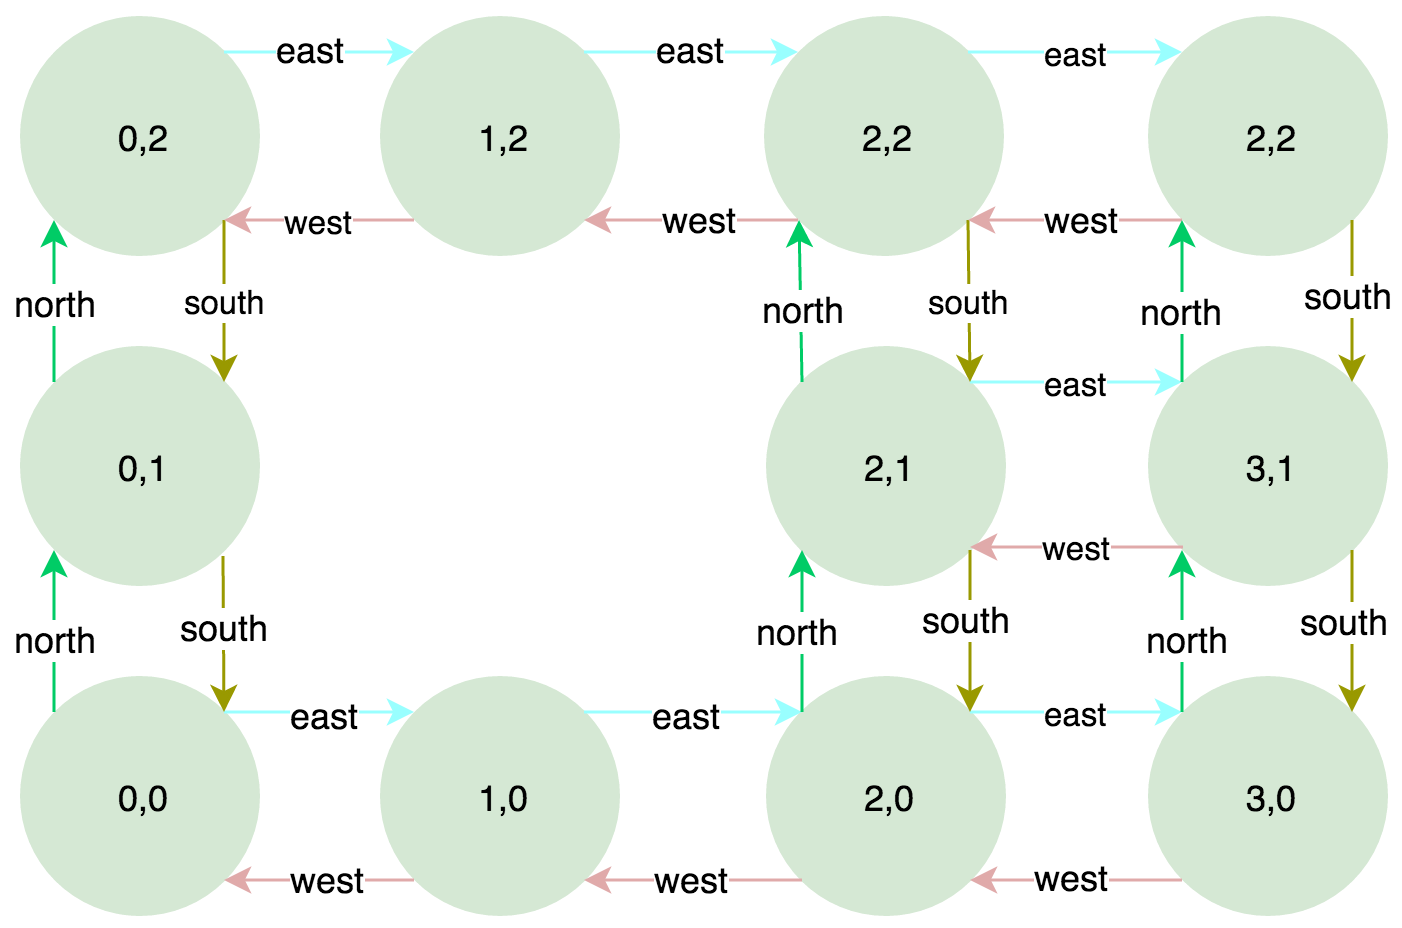
\includegraphics[width=.85\linewidth]{MDP_deterministic}
        \caption{Default grid}
        \label{fig:sub1}
    \end{subfigure}%
    \begin{subfigure}{.5\textwidth}
        \centering
        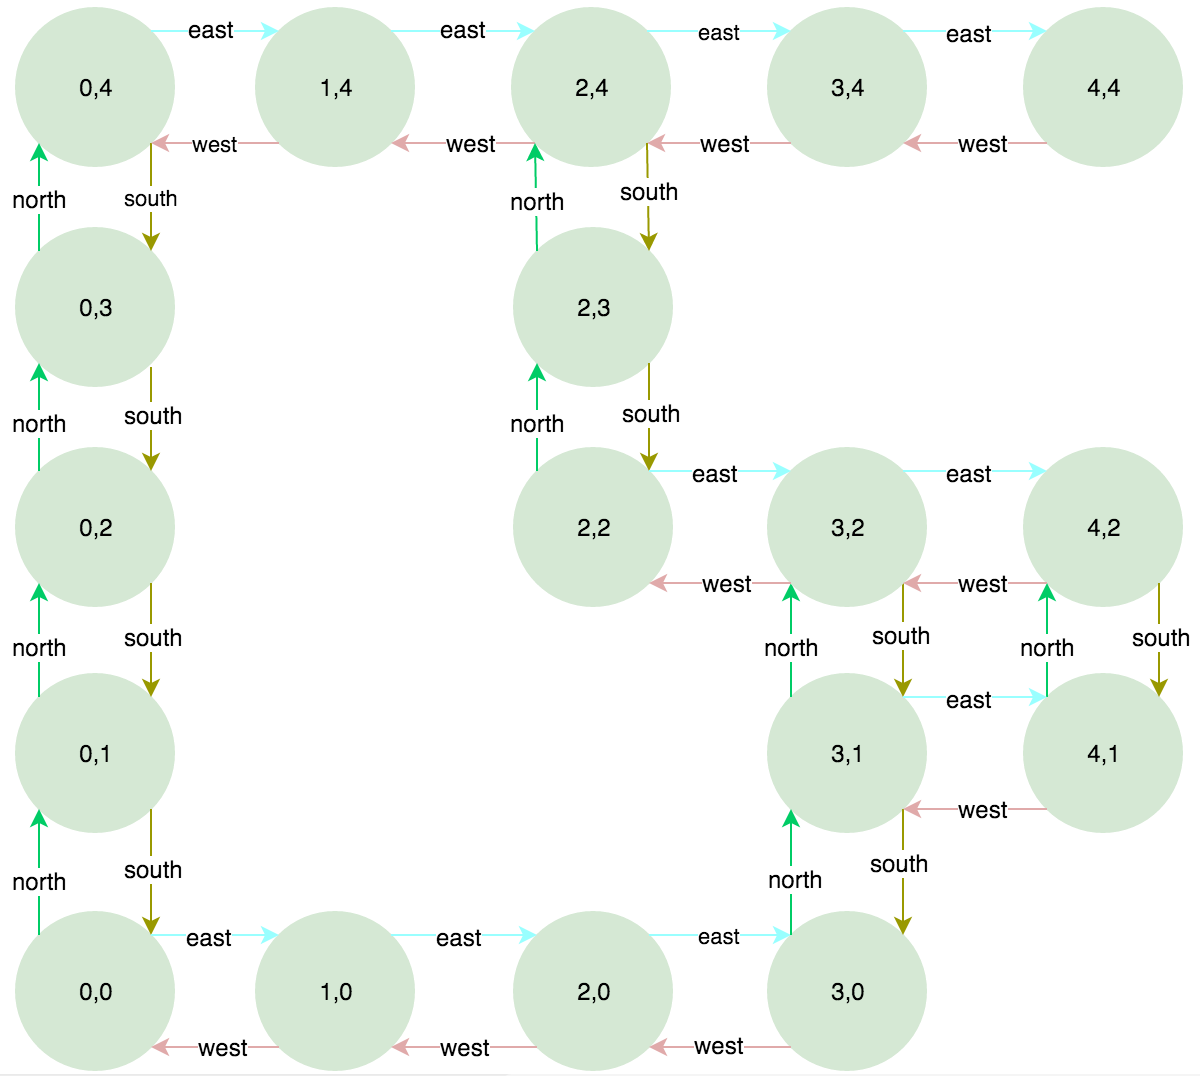
\includegraphics[width=.85\linewidth]{MDP_deterministic2}
        \caption{AAGrid}
        \label{fig:sub2}
    \end{subfigure}
    \caption{Deterministic MDPs}
    \label{fig:test}
\end{figure}

Estos laberintos, al igual que los demás incluidos en el código proporcionado, se almacenan en forma de arrays bidimensionales. Cada posición de la matriz representa una posición del laberinto, con los siguientes símbolos:
\begin{itemize}
    \item \textbf{Un espacio} representa una casilla común, sin recomensa ni coste algunos, por la que el agente puede pasar.
    \item \textbf{Un valor numérico} representa una casilla con una recompensa o un precio. Si el agente se mueve a esta casilla cambiará su puntuación añadiéndole el valor contenido en dicha casilla.
    \item \textbf{Una almohadilla (\#)} es considerada un muro, o casilla inalcanzable por el agente. Ninguna acción legal puede llevar al agente a estas posiciones.
    \item Por último, la posición de la que parte el agente se guarda como \textbf{una `S'}.
\end{itemize}

\newpage
\begin{wrapfigure}{r}{0.52\textwidth}
    \begin{verbatim}
          [[' ',' ',' ',' ',]
           ['8','#','3',' ',]
           ['#',' ',' ','#',]
           [' ',' ',' ',' ',]
           [' ','S','#',' ',]]
    \end{verbatim}
    \vspace{-20pt}
    \caption{New grid}
    \vspace{-10pt}
\end{wrapfigure}
De esta forma, podemos crear un nuevo laberinto siguiendo las instrucciones mencionadas. La siguiente figura muestra un laberinto creado por nosotros, en la que el agente deberá buscar una ruta sorteando los muros si quiere conseguir la mayor recompensa:\\[1em]

La elección de la política para guiar a un agente es clave para su éxito, y para ello se busca elegir la política óptima. Sin embargo, esta política no tiene por qué ser única y se caracteriza por compartir el mayor \textit{valor Q} de todas las políticas posibles. Así, para el laberinto por defecto tenemos dos políticas óptimas, las cuales muestra la figura a continuación.

\begin{figure}[h]
    \centering
    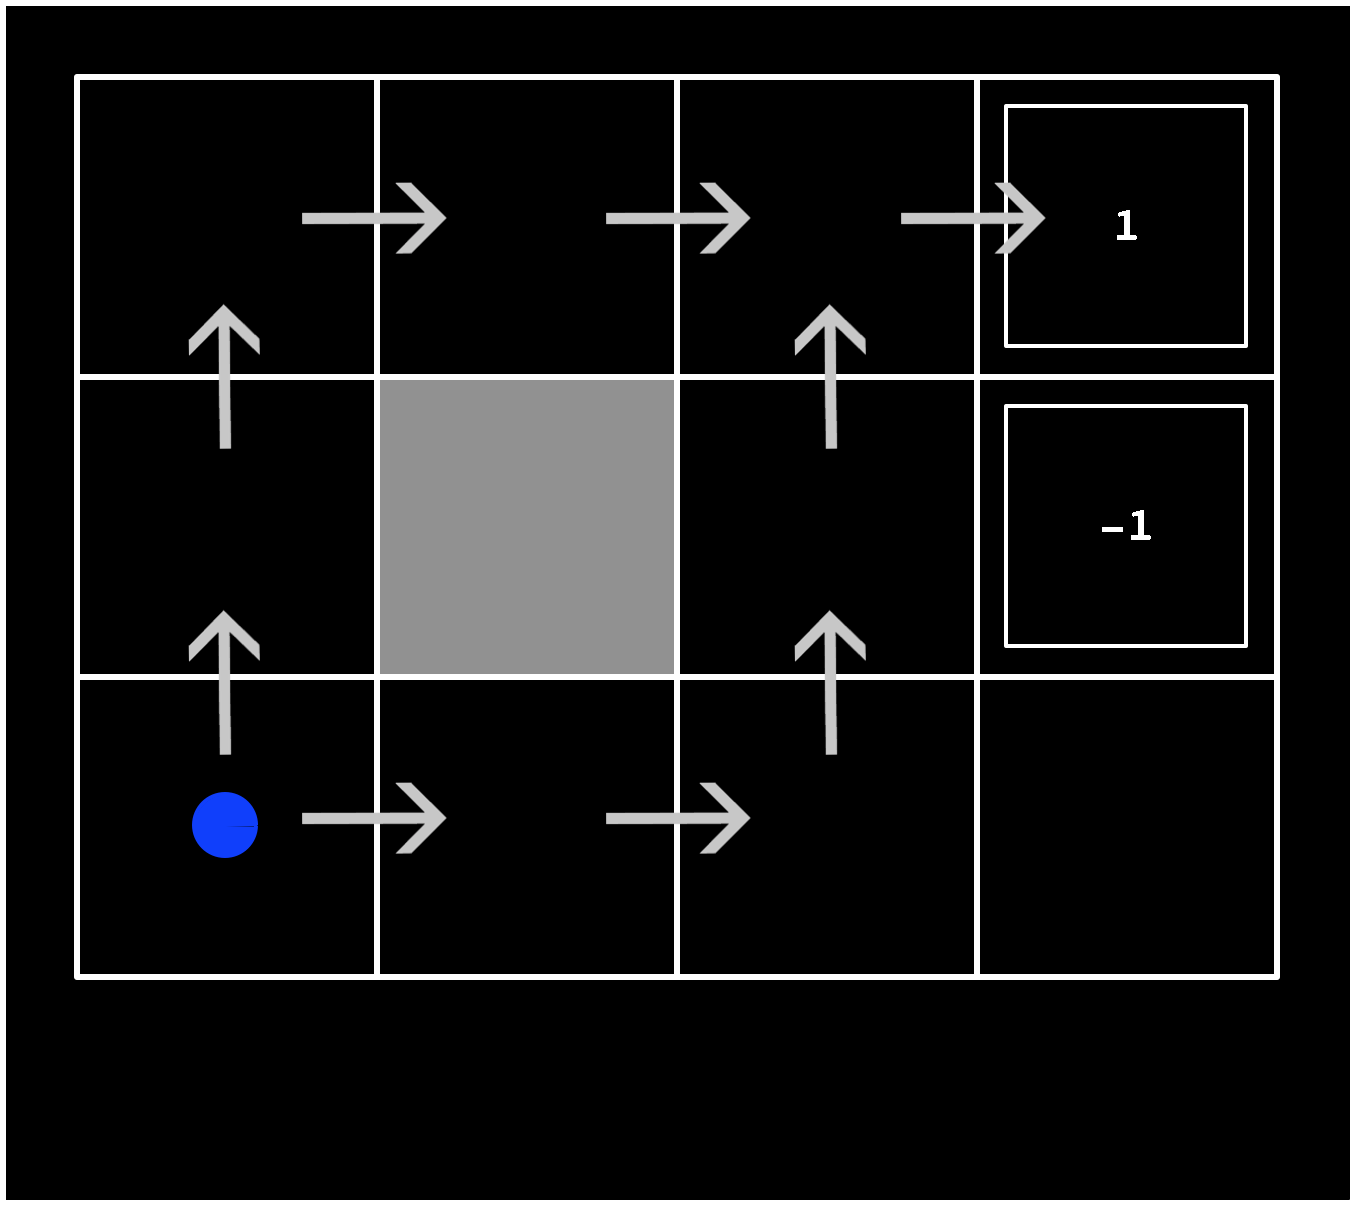
\includegraphics[width=8cm]{policies}
    \caption{Políticas óptimas para el laberinto por defecto}
\end{figure}

% https://webdocs.cs.ualberta.ca/~sutton/book/ebook/node41.html


\newpage
\section{Ejercicio 2}

En este ejercicio, implementamos el código necesario para que un agente automático fuese capaz de basar su política de acción en una \textit{tabla Q} dada a través de un fichero. Para ello:

\begin{itemize}
    \item El constructor de la clase inicializa los \textit{valores Q} a través de \texttt{readQtable}.
    \item \texttt{readQtable} guarda en un array \texttt{q\_table} los \textit{valores Q} de cada acción para cada uno de las acciones posibles desde el archivo donde se almacena dicha tabla.
    \item \texttt{writeQtable} actualiza el fichero con la actualizada \textit{tabla Q} tras la ejecución del juego.
    \item \texttt{computeActionFromQValues} devuelve, dado un estado, la acción con mayor \textit{valor Q} según la \textit{tabla Q} actual. De esta forma, devuelve la acción elegida por la política más avara de todas.
    \item \texttt{computeQValueFromQValues} devuelve, dado un estado, una acción y la \textit{tabla Q}, el \textit{valor Q} actual para dicha acción. Se tuvo que refactorizar el código para que el nombre de esta función fuese el mismo, dado que por defecto se denominaba \texttt{getQValue}.
\end{itemize}

Inicializamos la \textit{tabla Q} con todos los valores iguales a cero: \\

\begin{figure}[h]
    \centering
        \begin{tabular}{*{6}{c}}
            state \# & North & East & South & West & Exit\\
            0 & 0.0 & 0.0 & 0.0 & 0.0 & 0.0 \\
            1 & 0.0 & 0.0 & 0.0 & 0.0 & 0.0 \\
            2 & 0.0 & 0.0 & 0.0 & 0.0 & 0.0 \\
            3 & 0.0 & 0.0 & 0.0 & 0.0 & 0.0 \\
            4 & 0.0 & 0.0 & 0.0 & 0.0 & 0.0 \\
            5 & 0.0 & 0.0 & 0.0 & 0.0 & 0.0 \\
            6 & 0.0 & 0.0 & 0.0 & 0.0 & 0.0 \\
            7 & 0.0 & 0.0 & 0.0 & 0.0 & 0.0 \\
            8 & 0.0 & 0.0 & 0.0 & 0.0 & 0.0 \\
            9 & 0.0 & 0.0 & 0.0 & 0.0 & 0.0 \\
            10 & 0.0 & 0.0 & 0.0 & 0.0 & 0.0 \\
            11 & 0.0 & 0.0 & 0.0 & 0.0 & 0.0 \\
        \end{tabular}
    \caption{Initial Q table}
    \label{fig:test}
\end{figure}

% https://webdocs.cs.ualberta.ca/~sutton/book/ebook/node65.html
\newpage
\section{Ejercicio 3}

% TODO: Meter aquí todo lo de n = 0.3

En este ejercicio generamos una nueva \textit{tabla Q}, esta vez con un MDP estocástico. Tan estocástico que, una vez decidida la acción a tomar, hay menos posibilidades de que tome dicha posibilidad frente a que tome una acción adyacente. Esto es debido al ruido inducido del 0.9, causando que la probabilidad de que la acción elegida sea la ejecutada se reduzca a un ínfimo 10\%. La figura a continuación muestra el MDP resultante de este ruido:

\begin{figure}[h]
    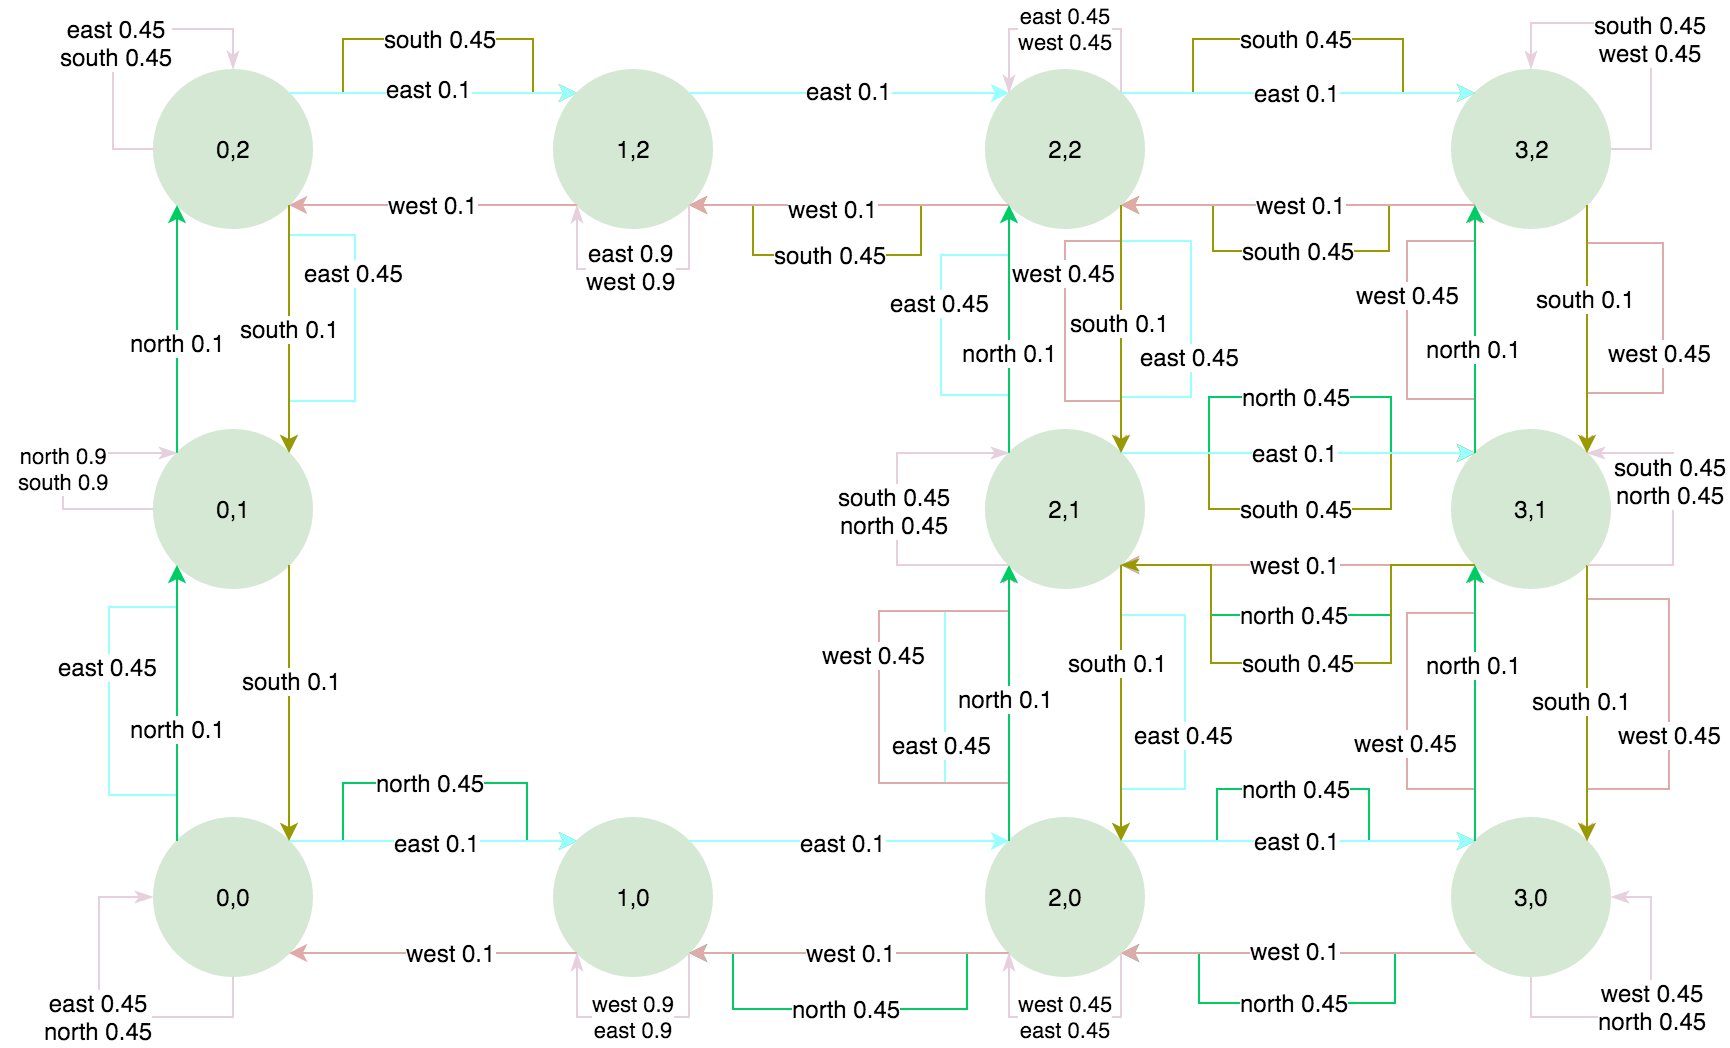
\includegraphics[width=\textwidth]{MDP_stochastic_09}
    \caption{MDP estocástico}
\end{figure}

Para elaborar dicho MDP, se ha tenido en cuenta varias consideraciones
\begin{itemize}
    \item Dada una acción, nunca se realizará la acción opuesta: eligiendo Norte nunca se tomará Sur, eligiendo Este nunca se tomará Oeste, y viceversa en ambos casos.
    \item La probabilidad de tomar cada una de las dos acciones adyacentes en caso de no tomar la acción elegida será la misma. Así, si tanto Norte como Este como Oeste se encuentran entre las acciones legales de un estado y se elige Norte, las probabilidades de tomar cada una de las acciones serán 0.1, 0.45 y 0.45, respectivamente.
    \item Si una acción alternativa (adyacente) a la elegida no se encuentra entre las acciones legales para un estado determinado, el agente se queda parado.
\end{itemize}

Dado un MDP tan indeterminista, la política conseguida tras ejecutar el algoritmo de \textit{QLearning} tras jugar más de veinte mil partidas es confusa:

\begin{figure}[h]
    \centering
    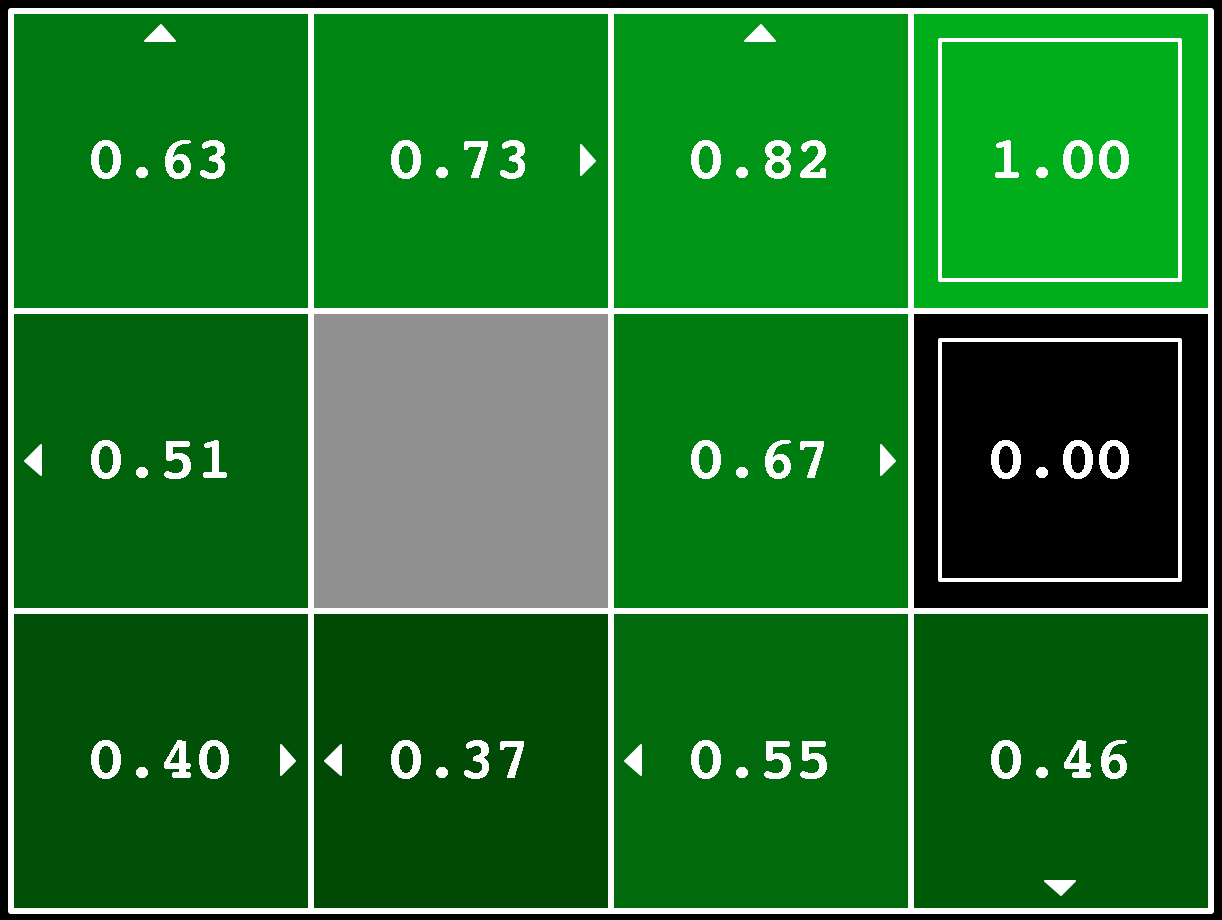
\includegraphics[width=0.5\textwidth]{policy_stochastic09}
    \caption{Política obtenida con el MDP estocástico}
\end{figure}

Para entender esta política aparentemente incorrecta, hace falta un análisis más en detalle. Como puede observarse, el agente trata de buscar la acción alternativa frente a la principal, ya que ha descubierto que es realizada con más frecuencia. Así, si quiere ir al Este elegirá la acción Norte o Sur, ya que sabe que de esta forma se moverá hacia la dirección que quiere con una probabilidad mucho mayor.

Tras explicar este enfoque, podríamos considerar la política del agente como óptima. Aún es más, si se observa la ejecución del agente se aprecia claramente cómo éste se desenvuelve con bastante soltura por el mapa y tiene unos resultados considerablemente satisfactorios, probando el razonamiento anterior.

Se puede entender que estas condiciones de aprendizaje son muy difíciles para el algoritmo, por lo que éste necesitará muchas más iteraciones para conseguir la política óptima que en los ejercicios anteriores.

\end{document}
